\chapter{Ellipsoidal Geometry}
\label{ch:ellipsoidal-geometry}

\subsection{Ellipsoid}
\label{sec:ellipsoid}
The shape of the ellipsoid is described by two geometric parameters, the 
\emph{semi-major} axis $\alpha$ and the \emph{semi-minor} axis $b$. $b$ is 
often replaced by the \emph{flattening} $f$, a smaller quantity describing the 
small polar flattening of the ellipsoid. $f$ is given by the formula:
\begin{equation}
  f = \frac{\alpha -b}{b}
  \label{eq:flattening}
\end{equation}

\subsubsection{Eccentricity}
\label{sssec:eccentricity}
The eccentricity can be expressed as:
\begin{equation}
  e = \sqrt{1 - \left( \frac{b}{a} \right)^2 }
    = \frac{\sqrt{\alpha ^2 - b^2}}{\alpha}
  \label{eq:eccentricity-1}
\end{equation}

Note that from \ref{eq:eccentricity-1}, we have:
\begin{equation}
  \sqrt{1-e^2} = \frac{b}{\alpha} = 1 - f
  \label{eq:eccentricity-2}
\end{equation}

\subsubsection{Ellipsoidal, Geocentric and Reduced Latitude}
\label{sssec:ellipsoidal-and-geocentric-latitude}

\begin{figure}
  \centering
\begin{tikzpicture}[line cap=round,line join=round]
  \pgfmathsetmacro{\rc}{4}
  \pgfmathsetmacro{\rb}{3.0}
  \pgfmathsetmacro{\xp}{2.2}
  \pgfmathsetmacro{\yp}{\rb * sqrt((1-(\xp * \xp)/(\rc *\rc))}
  \pgfmathsetmacro{\ecsq}{(\rc*\rc -\rb *\rb)/(\rc *\rc)}
  \tkzDefPoint(0,0){C}
  \tkzDefPoint(\rc,0){A}
  \tkzDefPoint(0,\rb){B}
  \tkzDefPoint(5,0){X}
  \tkzDefPoint(0,5){Y}
  \tkzDefPoint(\xp,\yp){P}
  \draw[name path=CX] (C)--(X);
  \draw[name path=CY] (C)--(Y);
  %\draw[name intersections={of=elip and AC, by={D}}];
  \tkzDrawPoints[fill=black](A,B,P)
  \tkzLabelPoints(A,B,P)
  \tkzFindAngle (A,C,B) \tkzGetAngle{an} \FPround\an\an{0} % 90 deg
  \pgfmathsetmacro{\ann}{atan2(sin(\an),cos(\an)/3)}
  \draw (A) arc (0:\ann:\rc cm and \rb cm);
  \draw (A) arc (0:\ann:\rc cm and \rc cm);
  \draw[name path=CP] (C)--(P); % geocentric
  \tkzMarkAngle[fill=yellow,
    size=0.4,
    opacity=0.4](A,C,P)
  \tkzLabelAngle[pos=.6](A,C,P){$\bar{\phi}$}
  \pgfmathsetmacro{\xpn}{\xp * \ecsq}
  \tkzDefPoint(\xpn,0){N}
  \draw[name path=NP] (N)--(P);
  \tkzMarkAngle[fill=red,
    size=0.4,
    opacity=0.8](A,N,P)
  \tkzLabelAngle[pos=.7](A,N,P){$\phi$}
  \pgfmathsetmacro{\ypc}{sqrt(\rc *\rc - \xp *\xp)}
  \tkzDefPoint(\xp,\ypc){M}
  \tkzDrawPoints[fill=black](M)
  \tkzLabelPoints(M)
  \draw[dashed, name path=PM] (P)--(M);
  \draw[dashed, name path=CM] (C)--(M);
  \tkzMarkAngle[fill=red,
    size=0.8,
    opacity=0.4](A,C,M)
  \tkzLabelAngle[pos=1.1](A,C,M){$\beta$}
  \draw [|<->|] ($(C)-(0,.2)$) -- node[below=1mm] {$\alpha$} ($(A)-(0,.2)$);
  \draw [|<->|] ($(C)-(.2,0)$) -- node[left=.3mm] {$b$} ($(B)-(.2,0)$);
  \tkzDefPoint(0,\rc){CB}
  \draw [|<->|] ($(C)-(.6,0)$) -- node[left=.5mm] {$\alpha$} ($(CB)-(.6,0)$);
\end{tikzpicture}
\caption{Ellipsoidal $\phi$, reduced $\beta$ and geocentric $\bar{\phi}$ latitude.}
\label{fig:latitudes}
\end{figure}

The \emph{geocentric} latitude $\bar{\phi}$, is related to the \emph{ellipsoidal} 
latitude $\phi$ (see \ref{fig:latitudes}) by the equation (\cite{Torge2001}, 
Section 4.1.1):
\begin{equation}
  \tan \bar{\phi} = \left( \frac{b}{\alpha} \right)^2 \tan \phi 
    = \left( 1 - e^2 \right) \tan \phi
\end{equation}

In \ref{fig:latitudes}, if we project (parallel to the $y$-axis) from point $P$ 
to the intersection of the coecentric circle (of radius $\alpha$), the geocentric 
angle obtained is labeled the \emph{reduced} latitude $\beta$. Reduced latitude 
can be expressed as a function of ellipsoidal latitude as (\cite{Torge2001}, 
Section 4.1.1):
\begin{equation}
  \tan \beta = \frac{b}{\alpha} \tan \phi = \sqrt{1-e^2} \tan \phi
  \label{eq:reduced-latitude}
\end{equation}

\begin{figure}
  \centering
  %\includegraphics[width=.65\linewidth, angle=-90]{Cryosat-2-RinexRfo}
  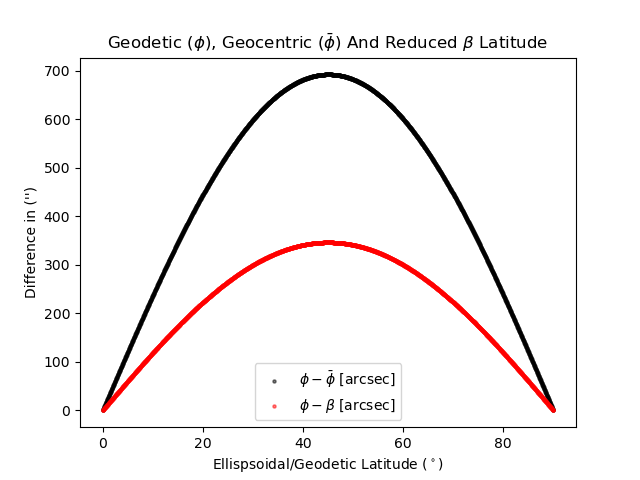
\includegraphics[width=.85\linewidth]{latitudes}
  \caption{Differences between ellipsoidal $\phi$, reduced $\beta$ and geocentric $\bar{\phi}$ latitude.}
  \label{fig:latitude-diffs}
\end{figure}

\begin{figure}
  \centering
\begin{tikzpicture}[line cap=round,line join=round]
  \pgfmathsetmacro{\rc}{4}
  \pgfmathsetmacro{\rb}{3.0}
  \pgfmathsetmacro{\xp}{2.2}
  \pgfmathsetmacro{\yp}{\rb * sqrt((1-(\xp * \xp)/(\rc *\rc))}
  \pgfmathsetmacro{\ecsq}{(\rc*\rc -\rb *\rb)/(\rc *\rc)}
  \tkzDefPoint(0,0){C}
  \tkzDefPoint(\rc,0){A}
  \tkzDefPoint(0,\rb){B}
  \tkzDefPoint(0,-\rb){Bm}
  \tkzDefPoint(5,0){X}
  \tkzDefPoint(0,5){Y}
  \tkzDefPoint(\xp,\yp){P}
  \draw[name path=CX] (C)--(X);
  \draw[name path=CY] (C)--(Y);
  %\draw[name intersections={of=elip and AC, by={D}}];
  \tkzDrawPoints[fill=black](A,B,P)
  \tkzLabelPoints(A,B,P)
  \tkzFindAngle (A,C,B) \tkzGetAngle{an} \FPround\an\an{0} % 90 deg
  \pgfmathsetmacro{\ann}{atan2(sin(\an),cos(\an)/3)}
  \draw (A) arc (0:\ann:\rc cm and \rb cm);
  \draw (A) arc (0:\ann:\rc cm and \rc cm);
  \draw[name path=CP] (C)--(P); % geocentric
  \tkzMarkAngle[fill=yellow,
    size=0.4,
    opacity=0.4](A,C,P)
  \tkzLabelAngle[pos=.6](A,C,P){$\bar{\phi}$}
  
  \pgfmathsetmacro{\xpn}{\xp * \ecsq}
  \pgfmathsetmacro{\ypn}{-\yp * (\rc * \rc - \rb * \rb)/ (\rb *\rb )}
  \tkzDefPoint(\xpn,0){N}
  \tkzDefPoint(0,\ypn){Nn}
  \tkzDefPoint(\rc,\ypn){An}
  \draw[name path=NNn] (P) -- (Nn);
  \draw[dashed] (Nn) -- (An);
  \tkzMarkAngle[fill=red,
    size=0.4,
    opacity=0.8](An,Nn,N)
  \tkzLabelAngle[pos=.7](An,Nn,N){$\phi$}
  \tkzMarkAngle[fill=red,
    size=0.4,
    opacity=0.8](A,N,P)
  \tkzLabelAngle[pos=.7](A,N,P){$\phi$}
  
  \pgfmathsetmacro{\ypc}{sqrt(\rc *\rc - \xp *\xp)}
  \tkzDefPoint(\xp,\ypc){M}
  \tkzDrawPoints[fill=black](M)
  \tkzLabelPoints(M)
  %\draw[dashed, name path=PM] (P)--(M);
  %\draw[dashed, name path=CM] (C)--(M);
  %\tkzMarkAngle[fill=red,
  %  size=0.8,
  %  opacity=0.4](A,C,M)
  %\tkzLabelAngle[pos=1.1](A,C,M){$\beta$}
  
  \draw [|<->|] ($(C)-(0,.2)$) -- node[below=1mm] {$\alpha$} ($(A)-(0,.2)$);
  \draw [|<->|] ($(C)-(.2,0)$) -- node[left=.3mm] {$b$} ($(B)-(.2,0)$);
  \tkzDefPoint(0,\rc){CB}
  \draw [|<->|] ($(C)-(.6,0)$) -- node[left=.5mm] {$\alpha$} ($(CB)-(.6,0)$);
  \draw[name path=CBm] (C)--(Bm); % negative y
\end{tikzpicture}
\caption{Ellipsoidal $\phi$, reduced $\beta$ and geocentric $\bar{\phi}$ latitude.}
\label{fig:latitudes}
\end{figure}
